\documentclass{article}
\title{
    \LARGE Agile Working - Project idea\\[0.2em]
    \Large Pineapple Planner
}
\author{Max Sellick, Varvara Aladyina, Deinoras Krasauskas, Azhaf Kahn, Simon Ostini}
\date{February 2025}

\usepackage{graphicx}
\graphicspath{{images/}}

\usepackage{booktabs}

\usepackage{float}
\usepackage[utf8]{inputenc}
\usepackage[english]{babel}
\usepackage[style=ieee]{biblatex}
\addbibresource{references/references.bib}
\usepackage{csquotes}
\usepackage[utf8]{inputenc}
\usepackage{hyperref}
\hypersetup{
    colorlinks=true,
    linkcolor=black,
    filecolor=magenta,
    urlcolor=blue,
}
\usepackage{listings}
\usepackage{multirow, makecell}
\usepackage{pgfplots}
\pgfplotsset{compat=1.18}
\usepackage{caption}
\usepackage{calculator}
\usepackage{calculus}
\usepackage{geometry}
\geometry{
    a4paper,
    left=30mm,
    right=30mm,
    top=25mm,
    bottom=30mm,
    headheight={90pt},
}
\usepackage[shortlabels]{enumitem}

\usepackage{enumitem}
\usepackage{tabularx}
\usepackage{booktabs}

\addto\captionsenglish{\renewcommand{\listfigurename}{Plots}}
\addto\captionsenglish{\renewcommand{\listtablename}{Tables}}

\begin{document}
\begin{figure}[ht!]
  \minipage{0.76\textwidth}
  
\includegraphics[width=7cm]{images/hkr.png}
  \label{title}
  \endminipage
  \minipage{0.32\textwidth}
  \endminipage
\end{figure}

\vspace{0.8cm}
\large

\textbf{{\let\newpage\relax\maketitle}}

\begin{center}
  \vfill
  \small{Kristianstad University | SE-291 88 Kristianstad | +46 44 250 30 00 | www.hkr.se}
\end{center}

\thispagestyle{empty}

\newpage

\makeatletter
\renewcommand{\abstractname}{\vspace{-\baselineskip}}
\begin{abstract}
  \large
  \noindent\textbf{Title}\\
  Agile Working - Project idea\\[1em]
  \textbf{Programme}\\
  Software Development\\[1em]
  \textbf{Authors}\\
  Max Sellick, Varvara Aladyina, Deinoras Krasauskas, Azhaf Khan, Simon Ostini\\[1em]
  % Abstract\\[1em]
  \textbf{Keywords}\\
  Agile, Scrum, Project idea\\[1em]
\end{abstract}
\makeatother

\newpage

\tableofcontents
\thispagestyle{empty}

\newpage

\section{Task 1}
This report focuses on our task management project "Pineapple Planner".
It is a task management tool with integrated calendar, todo list which aims to minimize stress in order to help completing daily tasks and improves personal productivity.
We are going to build a desktop application.
Our application aims to contribute to structure peoples lives and to help them achieve their daily goals.

\section{Task 2}
Considering ethical aspects and social responsibility in the development of the Pineapple Planner desktop application is crucial to ensure fairness, accessibility, and user trust.
Ethical principles help create a product that respects user privacy and promotes inclusivity.

One key consideration is data privacy and security.
Task management applications often store sensitive personal information, so implementing strong data protection measures aligns with ethical guidelines such as the General Data Protection Regulation.
Ensuring that user data is stored securely in a Firebase store and not exploited for commercial gain fosters trust and transparency.
\cite{hoofnagle2019european}

Additionally, our application should not include any manipulative design or addictive features that could pressure users.
\cite{montag2019addictive}


\section{Task 3}
\begin{enumerate}[a)]
  \item We plan to develop the Pineapple Planner app with scalability and usability in mind.
        By using Domain-Driven Design (DDD) with C\verb|#|, WPF, and Blazor, the system will be modular and easy to maintain, allowing the integration of new features over time if required.
        The combination of WPF for desktop and Blazor for web components will ensure a user-friendly and responsive interface.
        Technically, our infrastructure allows easy migration to cross-platform usage.
        With C\verb|#|’s strong type safety and GitHub’s CI/CD pipelines, the app will maintain data integrity and deliver stable updates.
        Lastly, we will strongly profit from JIRA's structured project and task management.
  \item We intend to build a C\verb|#| WPF application that integrates a Blazor web appplication as an external assembly.
        The Blazor app accesses data from a database through queries and commands (CQRS) which are implemented in the application layer assembly.
        The application layer accesses our entities that are defined in the domain layer.
        Generally, it can be said that we plan to use a microservice architecture according to the Domain-Driven-Design (DDD) infrastructure pattern also known as the \textit{Onion architecture}.
\end{enumerate}
\begin{figure}[t!]
  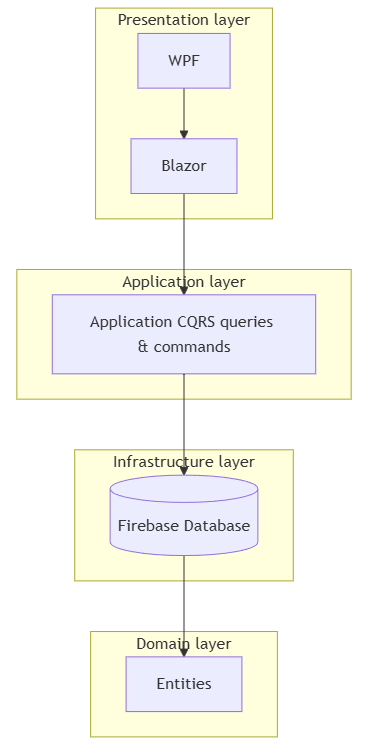
\includegraphics{images/infrastructure-proposal.png}
  \label{Infrastructure proposal}
  \caption{Infrastructure proposal}
\end{figure}
\clearpage

\section{Task 4}

R2. \\
D2. A task form allows the users to create, edit and delete their tasks.
\\[1em]
R3. The user link their task data to their account.\\
D3. The application saves a users' tasks in a database.\\

\begin{table}[h]
  \centering
  \begin{tabularx}{\textwidth}{l|X|l}
    \toprule
    \textbf{Nr} & \textbf{Requirement item}                          & \textbf{Priority (High/Medium/Low)} \\
    \hline\hline
    R1          & The user shall be able to inspect their tasks.     & High                                \\
    \hline
    R2          & The user shall be able to manage their tasks.      & High                                \\
    \hline
    R3          & The user link their task data to their account.    & High                                \\
    \hline
    R4          & The user shall be able to prioritize tasks.        & Medium                              \\
    \hline
    R5          & The user shall be able to set recurring tasks.     & Medium                              \\
    \hline
    R6          & The user shall be able to set reminders for tasks. & Low                                 \\
    \bottomrule
  \end{tabularx}
  \caption{Requirement items}
  \label{Requirement items}
\end{table}

\begin{table}[h]
  \centering
  \begin{tabularx}{\textwidth}{l|X|l}
    \toprule
    \textbf{Nr} & \textbf{Requirement item}                                                 & \textbf{Priority (High/Medium/Low)} \\
    \hline\hline
    D1          & Task items are listed in a todo list view and visible in a calendar view. & High                                \\
    \bottomrule
  \end{tabularx}
  \caption{Design items}
  \label{Design items}
\end{table}

\clearpage

\section{Task 5}

\begin{table}[h]
  \centering
  \begin{tabularx}{\textwidth}{l|X|X|X|X}
    \toprule
    \textbf{Sprint}       & Sprint 1                          & Sprint 2                          & Sprint 3                          & Sprint 4                          \\
    \hline\hline
    \textbf{Scrum master} & Varvara Aladyina                  & Deinoras Krasauskas               & Azhaf Khan                        & Max Sellick,\newline Simon Ostini \\
    \hline
    \textbf{Developers}   & Max Sellick,\newline Simon Ostini & Varvara Aladyina                  & Deinoras Krasauskas               & Azhaf Khan                        \\
    \hline
    \textbf{Tester}       & Deinoras Krasauskas               & Azhaf Khan                        & Max Sellick,\newline Simon Ostini & Varvara Aladyina                  \\
    \hline
    \textbf{Support}      & Azhaf Khan                        & Max Sellick,\newline Simon Ostini & Varvara Aladyina                  & Deinoras Krasauskas               \\
    \bottomrule
  \end{tabularx}
  \caption{Sprint role planning}
  \label{Sprint role planning}
\end{table}

\clearpage

\section{References}
\printbibliography[heading=none]

\end{document}
